

\section{Introduction}



It is well know that conventional accurate analog simulation tools, which are based on the Newton-Raphson nonlinear solver, can have serious drawbacks when they are used for the integration of non-smooth circuits, containing switches and piecewise linear components (like ideal diodes and transistors). This is especially true when the number of events becomes too large, or when sliding modes exist, which is common in practice. Then analog (SPICE-like) tools  may become very time consuming, or provide very poor results with chattering \cite{galias2006}, or even fail \cite{maffezzoni2006,yuan2003,mayaram2000,chung1994,biolek2007}. The same applies to ``hybrid'' integrators that consider an exhaustive enumeration of all the system's modes, which have a very limited scope of application because of the exponential growth of the number of modes that have to be simulated separately. Along the same lines, event-driven schemes can hardly simulate systems with large number of events, because they soon become quite time-consuming and do not allow for accumulations of events \cite{acary-brogliato2008}. 

It is therefore clear that other types of numerical schemes have to be applied for highly non-smooth switching circuits. Since a numerical method always relies on a specific modelling approach, a logical path is to first reconsider the models of non-smooth components (diodes, switches, transistors, {\em etc}) so that efficient numerical solvers can be applied. The non-smooth dynamical systems (NSDS) approach, which is the one chosen in this paper, appears to be a suitable framework for the simulation of non-smooth circuits, allowing one to efficiently simulate systems with very large number of events, and sliding mode trajectories. It consists of modelling non-smooth components as piecewise linear functions, with possible vertical branches (inducing some unilaterality in the system, hence possible state jumps, when these branches are infinite). The time-discretization of such non-smooth systems then yields various types of so-called one-step-non-smooth-problems (OSNSP), for instance complementarity problems or quadratic programs with equality-inequality constraints, which require specific solvers. The NSDS approach may then take advantage of the quite important works that have been led by the Nonlinear Programming community concerning the development of efficient solvers for complementarity problems \cite{facchinei} and optimization tools \cite{hiriart1992}, and also by the Contact Mechanics community \cite{acary-brogliato2008}, where Moreau and Jean developed the so-called Non-Smooth Contact Dynamics (NSCD) method within the theoretical framework of Moreau's sweeping process \cite{moreau1988,jean1999,moreau1999}. The numerical method that is used in this paper, owes a lot to the NSCD method of mechanics, and will be named {\em Moreau's time-stepping scheme}. As alluded to above, non-smooth components are often represented with piecewise-linear functions, or with complementarity relations, or with inclusions into normal cones. The piecewise-linear modelling approach in non-smooth electrical circuits has been pioneered by Chua et al  in \cite{chua1978,chua1983,chua1985}, and complementarity problems have been introduced in \cite{bokhoven1978,stevens1981,vandenberghe1989}, followed by the works of Leenaerts and van Bokhoven \cite{leenaerts1999,leenaerts-bokhoven1998}, Vlach et al \cite{bedrosian1992,vlach1997,vlach1995a,vlach1995b}. Camlibel et al \cite{frasca2008,camlibel2002} studied the convergence of backward Euler methods, and comparisons with other (analog and hybrid) integrators are proposed in \cite{vasca2009}. Glocker et al \cite{glocker2005,moller2007} led interesting developments showing the analogy between mechanics and electricity for various types of non-smooth components, and also proposed a time-stepping method inspired by Moreau's algorithm for contact mechanics (consequently quite close to the algorithm used in this paper). Variational inequalities of the second kind and electrical superpotentials  were recently introduced in electronics in \cite{adly2007,goelevenJOTA,addi2009} to study the existence and uniqueness of solutions for static circuits, or the equilibria of dynamical circuits with non-smooth devices. Other works may be found in \cite{enge2005,batlle2005,giaouris2008}.


The objective of this paper is twofold: first it is shown on an academic example taken from \cite{maffezzoni2006} that the NSDS approach allows one to simulate a non-smooth system for which conventional analog methods fail (roughly speaking, the iterative solver for complementarity problems converges, whereas Newton-Raphson's method does not); second, numerical results for a buck converter are presented and comparisons with other (analog and hybrid) tools are done. The buck converter example in fact demonstrates on a significant case study that the proposed time-stepping method is efficient for systems with a large number of events. Compared to previous works \cite{glocker2005,vasca2009}, the ideal switches are here modelled and simulated for the first time in a completely implicit way, the advantage of which will be explained.  The simulations are done with the {\sc siconos} software platform\footnote{http://siconos.gforge.inria.fr/} of the INRIA \cite{acary-brogliato2008,Acary-Perignon2007,mathmod}, that is an open-source software package dedicated to non-smooth dynamical systems described by complementarity relations. The paper is organized as follows: in section \ref{section2} the modelling and general time-discretization frameworks are recalled; in section \ref{section3} an elementary closed-loop switching circuit taken from \cite{maffezzoni2006} is simulated; in section \ref{section4} the buck converter example is treated and comparisons are presented. Conclusions end the paper. 


\textbf{Notation:} The following tools will be used in this paper. Let $K \subseteq \RR^{n}$ be a non empty convex set. The normal cone to $K$ at $x \in \RR^{n}$ is $N_{K}(x)=\{z \in \RR^{n} | \langle z, \zeta-x \rangle \leq 0\;\mbox{for all}\;\zeta \in K\}$. The projection in the euclidean metric of a vector $x \in \RR^{n}$ onto $K$ is denoted as proj$[K;x]$. A singleton is denoted as $\{t\}$. the identity matrix of $\RR^{m \times m}$ is denoted by $\mathsf I_m$ and the zero vector in $\RR^m$ by $0_m$.

The following standard mathematical programming problems will be used throughout this paper.
\begin{definition}[Variational Inequality (VI)\cite{facchinei}]
  Given a function $\mathsf F : \RR^p \rightarrow \RR^p$, and $X$ a non empty subset of $\RR^p$, the Variational Inequality (VI) problem is to find a vector $z\in \RR^p$ such that
  \begin{equation}
    \label{eq:vi}
    \mathsf F^T(z)(y-z) \geq 0, \forall y \in X.
  \end{equation}\cqfd
\end{definition}
\begin{definition}[Inclusion into a normal cone to a convex set\cite{rockafellar}]
  Given a function $\mathsf F : \RR^p \rightarrow \RR^p$, and $K$ a non empty convex subset of $\RR^p$, the inclusion into a normal cone to a convex set problem is to find a vector $z\in \RR^p$ such that
  \begin{equation}
    \label{eq:inclusion}
    0 \ni \mathsf F(z) + N_K(z) 
  \end{equation}\cqfd
\end{definition}

If $K=X$ is a convex set, the inclusion~(\ref{eq:vi}) and the VI~(\ref{eq:vi}) are equivalent.

\begin{definition}[Mixed Complementarity Problem (MCP)\cite{Dirkse.Ferris1995}]
  The Mixed Complementarity Problem(MCP) is defined as follows. Given a function $\mathsf F : \RR^p \rightarrow \RR^p$, lower and
  upper bounds $l, u \in (\RR \cup \{+\infty, -\infty\})^p$, find $z \in \RR^{p}$, $w,
  v \in \RR^{p}_{+}$, such that:
  \begin{equation}\label{eq:MCP}\left\{
      \begin{array}{l}  
        \mathsf F(z) = w-v \\
        l \leq z \leq u, \quad
        (z-l)^{T}w=0,\quad
        (u-z)^{T}v=0
      \end{array}\right.
  \end{equation}\cqfd
\end{definition}
Notice that a solution to the MCP satisfies the inclusion $-F(z) \in N_{[l,u]}(z)$.

\begin{definition}[Mixed Linear Complementarity Problem (MLCP)]
The Mixed Linear Complementarity Problem (MLCP) is defined by a MCP for which $\mathsf F$ in (\ref{eq:MCP}) is affine, \textit{i.e.} $F = M z +q$ for some matrix $M \in RR^{ p \times p}$ and some vector $q\in\RR^m$.\cqfd
\end{definition}

\section{The non-smooth dynamical systems approach to electrical circuits.}
\label{section2}

\subsection{Non-smooth electronic devices modelling}
\label{section21}

The NSDS approach for the  modelling of piecewise linear components in electrical circuits has been described in detail  in several of the above cited publications \cite{acary-brogliato2008,glocker2005,moreau1988,jean1999,moreau1999}, and will just be recalled here for the sake of readability. The NSDS approach is a package that consists of: a) non-smooth models, b) Moreau's time-stepping algorithm, c) OSNSP solvers. The current-voltage law of non-smooth electronic devices  may all be represented as inclusions into a normal cone to a convex set $K$, $0 \in \Phi(y,\lambda,t) + N_{K}(\lambda)$, where $\Phi(\cdot)$ is a function, $y$ and $\lambda$ are implicitly defined from $0=H(X,\lambda,t)$ and $y=G(X,\lambda,t)$ for some functions $H(\cdot)$ and $G(\cdot)$, and $X$ is the state vector of the circuit, composed of branch voltages and currents. A crucial point for simulation efficiency, however, is to keep as less slack variables as possible in the device representation. In addition some efficient OSNSP solvers as they will be described in Section~\ref{Sec:ONSNP-solvers} use directly such inclusions into a normal cone to a convex set, or the equivalent VI formulation. This is the case for the direct MCP solver that we used in our simulations. Let us illustrate this on the above four examples (ideal diode, switch, transistor, comparator). Finally, it is noteworthy that the inclusion modelling of the devices allows for nonlinear characteristics which may not be represented by complementarity relations. 



\paragraph{Non-smooth  diodes}  The notation for the currents and the potentials at the ports of
the diode is depicted in figure \ref{fig:DIODE}. Four models of diodes are depicted in figure \ref{figdiodes}: the smooth exponential Shockley model in figure \ref{figdiodes} (a), ideal diodes with possible residual current $-a$ and voltage $-b$ in figure \ref{figdiodes} (b), the ``hybrid'' model which considers the two modes separately with an associated script in figure \ref{figdiodes} (c), a piecewise-linear model in figure \ref{figdiodes} (d). The ideal diode model in figure  \ref{figdiodes} (b) is chosen in this paper. The drawbacks of the Shockley law is that it introduces stiffness in the dynamical equations. The hybrid model becomes rapidly unusable if the number $m$ of diodes increases, since the number of modes to be described in the associated script varies as $2^{m}$. This will be shown on the converter example. The model \ref{figdiodes} (d) leads a badly conditionned  algorithm  used to solve the OSNSP in section \ref{}. On the contrary the ideal model of figure  \ref{figdiodes} (b) yields, when introduced in the dynamics, well-conditioned complementarity problems, that yield time-stepping methods for which efficient solvers exist. Showing the efficiency of these methods is the object of this paper.


\begin{figure}
  \centering
  \input{./figure/diode.pstex_t}
  \caption{diode symbol.}
  \label{fig:DIODE}
\end{figure}

\begin{figure*}
  \subfigure[smooth modeling ]{
    \begin{minipage}{0.22\linewidth}
      \begin{center}
        \resizebox{\linewidth}{!}{\input{./figure/shockleylaw.pstex_t}}{
          \footnotesize $ i(t) = i_s \exp(- \frac{v(t)}{\alpha} - 1) $
        }
      \end{center}
      $ $ \\
    \end{minipage}
  }\hspace{-2mm}
  \subfigure[nonsmooth modeling]  
  {
    \begin{minipage}{0.22\linewidth}
      \begin{center}
        \resizebox{\linewidth}{!}{\input{./figure/figdiode.pstex_t}}
        \footnotesize $ 0\leq i(t)+a \perp v(t)+b \geq 0 $
      \end{center}  
      $ $ \\
    \end{minipage}
  } \hspace{-2mm}
  \subfigure
  [hybrid modelling 
  ]
  {%
    \begin{minipage}{0.22\linewidth}
      \begin{center}
        \resizebox{\linewidth}{!}{\input{./figure/hybrid_diode.pstex_t}}\\
        \footnotesize $\begin{array}{cll}
          \mathsf{off} &=& \mathsf{s} < 0 \\
          v(t)  &=& \mathbf{if}\quad \mathsf{off} \quad \mathbf{then}\quad \mathsf{-s} \\
          & & \quad \mathbf{else} \quad 0 \\
          \ i(t) &=& \mathbf{if}\quad \mathsf{off} \quad
          \mathbf{then}\quad 0 \\
          & & \quad \mathbf{else}\quad \mathsf{s}
        \end{array} $ %
      \end{center}
      $ $ \\
       \end{minipage}
}
      \subfigure[equivalent resistor model]{
        \begin{minipage}{0.22\linewidth}
          \begin{center}
            \resizebox{\linewidth}{!}{\input{./figure/diodeReq.pstex_t}} \\
            { \footnotesize $v(t)=\begin{cases}-R_\on\; i(t) & \mbox{if}\;v(t) < 0 \\   -R_\off\; i(t) & \mbox{if}\;v(t) \geq  0 \\ R_\on \ll 1 & R_\off \gg 1 \end{cases}$ }\\
          \end{center}
          $ $ \\
        \end{minipage} }
      \caption{four models of diodes.}
\label{figdiodes}
\end{figure*}



Quite similar developments and comments may be made for ideal Zener diodes, piecewise linear practical diodes and practical Zener diodes, see e.g. \cite{acary-brogliato2008,addi2009}. From basic convex analysis one deduces that the ideal diode of figure \ref{figdiodes} (b) has the following current/voltage law: 

\begin{equation}\label{includiode}
i(t) \in \{b\}+N_{]-\infty,a]}(v(t))\;\Leftrightarrow \; v(t) \in \{a\}+N_{]-\infty,b]}(i(t))
\end{equation} 

Similar inclusions for ideal Zener diodes may be found in \cite{acary-brogliato2008,addi2009}, that take the form $i(t) \in N_{[0,V_{z}]}(v(t))$ for some $V_{z} >0$. The piecewise-linear  diode of figure \ref{figdiodes} (d) can be represented as:
%%
\begin{equation}\label{includiode2}
\left\{\begin{array}{l}
v(t)=\frac{1}{2}(\tau(t)-1) R_\off i(t) -\frac{1}{2}(1+\tau(t)) R_\on i(t) \\ \\ \tau(t) \in \mbox{sgn}(v(t))\; \Leftrightarrow \; v(t) \in - N_{[-1,1]}(\tau(t))
\end{array}\right.
\end{equation}
%%
that is consistent with the MLCP formulation in (\ref{MLCP}). The piecewise-linear model yields a condition number of the resulting MLCP matrix close to $\frac{R_\off}{R_\on}$, that causes trouble with the numerical algorithms that are used to solve the OSNSP. Inclusion as in (\ref{includiode}) will be preferred as it can be directly used in the numerical algorithm for MCP, yielding well-posed and well-conditioned MCPs. 



\paragraph{Non-smooth switches}  The notation for the currents and the potentials at the ports of the ideal switch is depicted on figure \ref{fig:IDEAL_SWITCH}. The switches are modelled in two ways in this paper. The first model, that is applied to the elementary example of section \ref{section3}, consists of:
%%
\begin{equation}\label{switchmodel1}
v(t)=\left\{\begin{array}{ll} R_\off\; i(t) & \mbox{if}\;u_{c}(t) < 0 \\   R_\on\; i(t) & \mbox{if}\;u_{c}(t) \geq  0  \end{array}\right.
\end{equation} 
%%
where the voltage $u_{c}(\cdot)$ is a state variable of the overall dynamical system, $v(\cdot)$ is the voltage of the switch and $i(\cdot)$ is the current through the switch. The resistors $R_\off \gg 1$ and $R_\on \ll 1$ are chosen by the designer. In the case of the buck converter of section \ref{section4}, the switch is modelled with transistors, as is most common in the industrial practice. The switch in (\ref{switchmodel1}) is modeled as follows:
%%
\begin{equation}
  \label{eq:63switch}
\left\{\begin{array}{l}
v(t)=\frac{1}{2}(1+\tau(t))R_\on i(t)+\frac{1}{2}(1-\tau(t))R_\off i(t)  \\ \\ \tau(t) \in \mbox{sgn}(u_{c}(t)) \; \Leftrightarrow \; u_{c}(t) \in -N_{[-1,1]}(\tau(t))
\end{array}\right.
\end{equation}
%%
The difference with respect to the diode (\ref{includiode2}) is that the ``input'' to the inclusion is an external voltage. It is noteworthy that the model in (\ref{switchmodel1}) is discontinuous at $u_{c}(t)=0$ for any $i(t) \not = 0$, the jump magnitude being equal to $|(R_\off-R_\on)i(t)|$. The choice that is made in (\ref{eq:63switch}) implies that the discontinuities are ``filled-in'' and the model is consequently multivalued at $u_{c}(t)=0$,  $i(t) \not = 0$. This is precisely what allows one to smoothly simulate the sliding-modes \cite{Acary.Brogliato2009}. 



\begin{figure}
  \centering
  \scalebox{0.7}{
  \input{./figure/IdealSwitch.pstex_t}
  }
  \caption{Ideal switch symbol.}
  \label{fig:IDEAL_SWITCH}
\end{figure}
 



\begin{remark}
  The  ideal switch is modelled in \cite{glocker2005} with a relay multifunction whose threshold may vary between 0 and $+\infty$, and the switch is controlled by a current variable of the circuit, in an explicit way. Compared to \cite{vasca2009} our approach differs a lot since \cite{vasca2009} models the switch through a so-called cone complementarity problems, with an exogenous excitation that makes the cones switch between $\{0\}$ and $\RR$ or $\RR^{+}$. The choice we made in this paper is motivated by the industrial practice and the way switches are modelled in Mentor Graphics' {\sc eldo} software package\footnote{\url{http://www.mentor.com/products/ic$\_$nanometer$\_$design/analog-mixed-signal-verification/eldo/}}, that is one of the main analog simulation tool of the market and may be considered as a reference for simulation results comparisons. Another way to model switches is to compute the topology changes after each ``open'' and ``close'' operation. As pointed out above such an approach rapidly becomes extremely time-consuming when the number of switches grows (the number of different topologies grows exponentially fast with the number of switches), and does not allow for finite accumulations of switches or sliding mode trajectories. An open issue would be the implicit discretization of the ideal switches models of \cite{glocker2005} and \cite{vasca2009} which is directly possible and  not tackled in this paper. 
\end{remark}


\paragraph{Non-smooth MOSFET transistors}  Following \cite{leenaerts-bokhoven1998}, let us consider the Sah model of the nMOS static characteristic:
\begin{equation}
  \label{eq:MOS_LEE_VAN}
I_{DS} = \frac{K}{2} \cdot (f(V_G-V_S-V_T) - f(V_G-V_D-V_T))
\end{equation}
with $K = \mu\Frac{\epsilon_{OX}}{t_{OX}}\Frac{W}{L}$ and  $\mu$ mobility of majority carriers, $W$ and $L$ channel width and length, $\epsilon_{OX}$ the permissivity of the silicon oxide of thickness $t_{Ox}$. The voltage $V_T$ is the threshold voltage depending on the technology. 

 The notation for the currents and the potentials at the ports of the nMOS is depicted on figure \ref{fig:NMOS}. The function $f :\mathbb{R} \longrightarrow \mathbb{R}$ in (\ref{eq:MOS_LEE_VAN}) is defined as:
\[
f(x) = \left\{ \begin{array}{ll}
0 & \textrm{if $x < 0$}\\
x^2 & \textrm{if $x \geq 0$}
\end{array} \right.
\]
The piecewise and quadratic nature of this function is approximated by the following $s$ segments piecewise linear function in \cite{leenaerts-bokhoven1998}: 
\begin{equation}\label{eq:pwl}
f_\pwl(x) = \alpha_i x + \beta_i, \text{ for } a_i \leq x \leq a_{i+1}, \quad i = -1\ldots s+1
\end{equation}
with $a_1 = -\infty$ and $a_{s+1} = +\infty$.
\begin{figure}
  \centering
  \input{./figure/nMOS.pstex_t}
  \caption{nMOS transistor symbol.}
  \label{fig:NMOS}
\end{figure}

The complete model of the piecewise-linear nMOS transistor with $s$ segments in (\ref{6segments}) can be recast under the following mixed linear complementarity form \cite{leenaerts-bokhoven1998}:
\begin{equation}
  \label{eq:68}
  \begin{array}{l}
    \begin{split}
      y(t) = \left[\begin{array}{cc} \underbrace{ \begin{array}{ccc}
              0 & \ldots & 0 \\
              -b & \ldots & -b
            \end{array}}_{\times s-1}
          &\underbrace{ \begin{array}{ccc}-b &\ldots & -b \\ 0 &\ldots & 0\end{array}}_{\times s-1} \\
        \end{array}\right]^T
      v(t) + \lambda(t) \\ + \left[\begin{array}{cccccc} h_1 &\ldots &
          h_{s-1} & h_1 &\ldots & h_{s-1}
        \end{array}
      \right]^T (t)
    \end{split}
\\ \\ 
 0 =
  \mathsf I_3\,
 i(t) 
 + 
 \left[\begin{array}{cccccc}
   -c_1  &\ldots & -c_{s-1} & c_1 &\ldots c_{s-1} \\
   0  & 0& 0 &0  & 0  \\
   c_{1}  &\ldots & c_{s-1} & -c_1 &\ldots -c_{s-1} \\
 \end{array}\right]
\lambda(t) \\ \\ 0 \leq y(t) \perp \lambda(t) \geq 0
\end{array}
\end{equation}
  with
\begin{equation}
  \label{eq:69}
  u(t) = 
  \left[\begin{array}{c}
    U_{GD}(t)=V_G(t)-v_D(t) \\
    U_{GS}(t)=V_G(t)-v_S(t) \\ 
  \end{array}\right],\quad\quad
i(t) = 
  \left[\begin{array}{c}
   I_D(t) \\
   I_G(t) \\
   I_S(t) \\
  \end{array}\right].
\end{equation}
The parameters are give as follows: $b = \frac{K}{2}$, $h_i = b(V_T+a_i), i =1\ldots 5 $. The values of $c_i$ are computed from the linear approximation $\alpha_i$ and $beta_i$ in (\ref{eq:pwl}). Using some basic convex analysis, one obtains the compact formulation of (\ref{eq:68}) (\ref{eq:69}): 
%%
\begin{equation}
\left\{\begin{array}{l}
-\lambda(t)+Bu(t)+h(t) \in N_{K}(\lambda(t))\; \Leftrightarrow  \;  \lambda(t)=\mbox{proj}[K; -Bu(t)-h(t)] \\[2mm]
y(t)=Bu(t)+\lambda(t)+h(t) \\[2mm]
0=i(t)+C\lambda(t)
\end{array}\right.
\end{equation}
%%
with $K=(\RR^{+})^{2(s-1)}$. In the case of the MOSFET transistor, the inclusion is an equality as expected since its piecewise-linear characteristic is single valued. The pMOS transistor is represented in the same way, changing the values of the $h_{i}(t)$, $i(t)$ to $-i(t)$ and $b$ to $-b$. 


\begin{remark}
The piecewise-linear model in (\ref{eq:pwl}) has $s$ segments. Multiple choices are possible in order to adjust the number of slack variables and consequently the size of the OSNSP-MLCP to be solved at each step with respect to the accuracy. As we will show in section \ref{section4} the numerical results are very little influenced by the reduction of number of segments. In practice one should therefore be very careful about choosing a reasonable piecewise-linear approximation of the devices so that the MLCP size does not increase too much. 
\end{remark}




\paragraph{Non-smooth comparator} The comparator device as depicted in figure \ref{} is a relay multifunction that is multivalued at 0. Other models can be chosen, see figure \ref{fig-comparator-models}. For the simulation of the buck converter in section \ref{section4}, we have chosen ????. Similarly to the Zener diode the multivalued comparator is represented as:

\begin{equation}
V_{output} \in N_{[V_{\min},V_{\max}]}(V_{+}-V_{-}) 
\end{equation}

\begin{ndrva}
  To do ...
\end{ndrva}

\subsection{The dynamical equations}
\label{section23}


Section \ref{section21} is devoted to present the electronic devices models and their mathematical representations to be inserted in the circuits dynamics in order to obtain a suitable formalism for subsequent time-discretization. In particular the OSNSP solver to be used strongly influences the modelling choice. In this section we focus on the dynamical equations which are suitable for the NSDS approach. 



\subsubsection{The non-smooth DAE formulation}


The extended MNA formulation with non-smooth components represented as inclusions and equalities, and nonlinear behavior can  be written compactly as:
\begin{equation}
  \label{eq:71}
 \left\{ \begin{array}{l l l}
    \begin{array}{l}
  M(X,t) \dot X = F(X,t) + U(t)
\end{array}
& & ]\text{ Differential Algebraic Equations (DAEs)}\\[2mm]
  \begin{array}{l}
    0 = H(X,\lambda,t)\\
    y = G(X,\lambda,t) 
  \end{array} &  & \bigg]\begin{array}{l}
   \text{Input/output relations }\\
   \text{on non-smooth components}
  \end{array}  \\[2mm]
  \begin{array}{l}
  0 \in \Phi(y,\lambda,t) + N_K(\lambda)
\end{array}
&  & ] \text{ "Inclusion rule"}\\ 
\end{array}\right.
\end{equation}
with $X \in \RR^n $ is  the state which is composed of the potentials, and the currents in inductive, voltage--defined and nonsmooth branches. The vectors $y,\lambda \in \RR^m$ are the slack variable expressing the nonsmooth multi-valued models of components. The functions $M : \RR^n\times\RR \rightarrow \RR^{p \times n}$, $H : \RR^n\times \RR^m\times\RR \rightarrow \RR^{n-p}$, $G : \RR^n\times \RR^m\times\RR \rightarrow \RR^{m}$ and  $\Phi : \RR^m\times \RR^m\times\RR \rightarrow \RR^{m}$ are assumed to be  continuously differentiable functions. More details will be given on the choice of state variables and the structure of the functions in Section~\ref{sec:acef}. One recognizes two basic ingredients: the DAE part, that is coupled to the non-smooth electronic devices represented by generalized equations as those developed in section \ref{section21}. See section \ref{section3} for a concrete example of (\ref{eq:71}). 


\subsection{Moreau's time-stepping scheme}


Starting from the dynamics in (\ref{eq:71}) the Moreau's time-stepping scheme  is as follows:
\label{section24}
\begin{equation}
  \label{eq:71-discrete}
 \left\{ \begin{array}{l}
    \begin{array}{l}
  M(X_{k+\theta},t_{k+\theta}) (X_{k+1}-X_{k}) = h F(X_{k+\theta},t_{k+\theta}) + h U(t_{k+\theta})
\end{array}\\[2mm]
  \begin{array}{l}
    0 = H(X_{k+1},\lambda_{k+1},t_{k+1})\\
    y_{k+1} = G(X_{k+1},\lambda_{k+1},t_{k+1}) 
  \end{array} \\[5mm]
  \begin{array}{l}
  0 \in \Phi(y_{k+1},\lambda_{k+1},t_{k+1}) + N_K(\lambda_{k+1})
\end{array} \\
\end{array}\right.
\end{equation}
for a time--step $h>0$ and with the usual following notation. For a function $f(t)$, $ f_{k+1} \approx f(t+1)$ and $f_{k+\theta} = \theta f_{k+1} + (1-\theta) f_{k}$. The Moreau's time stepping is made of a $\theta$-method for $\theta \in [0,1]$ for the assumed sufficiently smooth terms. and a fully implicit scheme for the inclusion rule which can be nonsmooth. This choice is led by two fundamental reasons. The first reason is the respect of the inclusion rule and its intrinsic unilateral character.  As it has been shown in \cite{Moreau1977},  only a fully implicit scheme can satisfied the unilateral constraints in discrete time. The second reason is the possible nonsmoothness of the evolution  which  can be only  numerically integrated by implicit low order schemes in a consistent way \cite{acary2008}.

For the numerical purposes, let us rewrite the problem~(\ref{eq:71-discrete}) in a global inclusion form
\begin{equation}
  \label{eq:inclusion-global}
    0 \ni \mathsf F(z) +N_{C}(z)
\end{equation}
where  the variable $z = [X_{k+1}, y_{k+1}, \lambda_{k+1}]^T \in \RR^{n+2m}$ and the function $\mathsf F : \RR^{n+2n} \rightarrow \RR^{n+2m} $ is defined by
\begin{equation}
  \label{eq:inclusion-global2}
  \mathsf F(z) =
  \left[\begin{array}{l}
      \begin{split}
        M(\theta X_{k+1}+(1-\theta)X_{k},t_{k+\theta}) (X_{k+1}-X_{k})\qquad\qquad \\
       - h F(\theta X_{k+1}+(1-\theta)X_{k},t_{k+\theta}) - h
        U(t_{k+\theta})
      \end{split}
\\
     H(X_{k+1},\lambda_{k+1},t_{k+1})\\
     G(X_{k+1},\lambda_{k+1},t_{k+1}) - y_{k+1} \\
     \Phi(y_{k+1},\lambda_{k+1},t_{k+1})
  \end{array}\right]
\end{equation}
The normal cone $N_C$ is the normal cone  to the following convex set
\begin{equation}
  \label{eq:inclusion-global3}
  C =  \RR^{n} \times \RR^ m \times K \subset \RR^{n+2m}
\end{equation}
We will see in the next section that the non linearity of $\mathsf F$ can be directly treated by the numerical one--step solver. Another approach is to performed an outer Newton linearization of this problem by searching the solution as the limit for $\alpha$ of the following linearized problem
\begin{equation}
  \label{eq:inclusion-global-linearized}
    0 \ni \mathsf \nabla_z\mathsf F(z^{\alpha})(z^{\alpha+1}-z^{\alpha}) + \mathsf F(z^{\alpha})  +N_{C}(z^{\alpha+1}).
\end{equation}
At each time--step, $k$ and at each Newton iteration $\alpha$, the problem appears to be affine in $z$.



\subsection{Numerical  solvers for the OSNSP~(\ref{eq:71-discrete})}
\label{Sec:ONSNP-solvers}
The problem~(\ref{eq:71-discrete}) appears to be a VI  written in the form of an inclusion into a normal cone to a convex set as in (\ref{eq:inclusion-global2}). The choice of the numerical solvers for~(\ref{eq:71-discrete}) depends mainly on the structure of the convex set $K$. Indeed, from a very general convex set $K$ to a particular choice of $K$, the numerical solvers range from the numerical methods for VI to nonlinear equations, passing through the various of complementarity problems solvers. More the structure of $K$ is simple, more the convergence and the numerical efficiency is improved.   In the sequel, majors choices of $K$ will be given leading to various classes of well-known problems in mathematical programming theory. We refer to \cite{facchinei} for a thorough presentation of available numerical solvers and to \cite[Chapter 12]{acary-brogliato2008}) for a comprehensive summary of numerical algorithms. In the numerical example presented in this paper, various numerical methods described below are used according to the type of the one--step nonsmooth problem and will be further precised. 



\subsubsection{$K$ is a finite representable convex set}
In practice, the convex set is finitely represented by
\begin{equation}
  \label{eq:K-finite}
  K = \{\lambda\in \RR^m, h(\lambda) = 0, g (\lambda) \geq 0 \},
\end{equation}
where the functions $h :  \RR^m \rightarrow \RR^m$, $g :  \RR^m \rightarrow \RR^m$ are assume to be smooth with non vanishing Jacobians. In this case, general algorithms for VI can be used. To cite a few of them, the minimization of the so-called  regularized gap function \cite{Fukushima1992,Zhu.Marcotte1993,Zhu.Marcotte1994}  or generalized Newton methods \cite[Chapter 7\& 8]{facchinei} can be used. If $F$ is affine (possibly after the linearization step described in (\ref{eq:inclusion-global-linearized}) ) and the function $h$ and $g$ are also affine, the VI is aid to be an affine VI for which the standard pivoting algorithms for LCP\cite{Cottle.Pang.ea1992} has been extended in \cite{Cao.Ferris1996}.

\subsubsection{$K$ is a generalized box}
Let us consider the case that $K$ is a generalized box in $\overline{\RR}^m =\RR \cup \{+\infty, -\infty\}^m$, that is
\begin{equation}
  \label{eq:K-box}
  K = \{\lambda\in \RR^m, a_i \leq \lambda _i \leq b_i, a_i \in \overline{\RR}, b_i\in \overline\RR, i = 1\ldots m \},
\end{equation}
In this case, the problem (\ref{eq:inclusion-global}-~(\ref{eq:inclusion-global3}))  can be recast in a Mixed Complementarity Problem (MCP) by defining $p=n+m+m+m$ and  the bounds $l,u$ as $l =[
\begin{array}{cccc}
0_n & 0_m & 0_m & a ]^T 
\end{array}
]^T$ and $u =[
\begin{array}{cccc}
0_n & 0_m & 0_m & b ]^T 
\end{array}]^T$.
 
The MCP (\ref{eq:MCP}) can be solved by a large family  of solvers based on Newton--type Methods and interior-points techniques. In contrast to the interior-point methods, it is not difficult to find comparisons of numerical methods based on Newton's method for solving MCP. We refer to the paper of \cite{Billups.ea1997} for an impressive comparison of the following implementation of solvers: MILES \cite{Rutherford1993}, PATH \cite{Dirkse.Ferris1995}, NE/SQP \cite{Gabriel.Pang1992,Pang.Gabriel1993}, QPCOMP \cite{Billups.Ferris1995}, SMOOTH \cite{Chen.Mangasarian1996}, PROXI \cite{Billups1995}, SEMISMOOTH \cite{Deluca.ea1996}, SEMICOMP \cite{Billups1995}. All of these comparisons, which have been made in the framework of the MCP~(\ref{eq:MCP}) show that the PROXI, PATH and SMOOTH are superior on a large sample of test problems.  For a comparison of the variants of the SEMISMOOTH algorithm,  we refer to \cite{DeLuca.Facchinei.ea2000}.

If $\mathsf F$ is affine, the problem is called Mixed Linear Complementarity Problem (MLCP) and we retrieve a box-constrained Affine VI. For this problem, standard pivoting algorithm such the Lemke's Method has been extended in~\cite{Sargent1978}.  

A special case of a generalized box is the positive orthant of  $\RR^m$, that is $K=\RR_+^m$. In this case, standard theory and most of the numerical algorithms LCP apply in this MCLP case. 

\section{Automatic circuit equation generation and Software implementation}

\subsubsection{Automatic generation of the dynamical equations}
\label{sec:acef}
\begin{ndrva}
  To do :
  \begin{itemize}
  \item Be more precise on the choice of variables. Introduce notation $I_{\mathsf L} \ldots$
  \item Do we need to speak about the reduction to a semi-DAE ?
  \end{itemize}
\end{ndrva}


Let us describe briefly how the dynamical equations are obtained for the two systems which are analyzed in this paper. There are basically three choices for the state variables, based on the charge approach, the flux approach, and the current-voltage approach. The latter is chosen here. An automatic circuit equation generation system has been developed at the INRIA, see the patent \ref{}.  There are a lot of methods to build a non-smooth DAE formulation. Indeed, all smooth formulations (STA or MNA) could be adapted by replacing the constitutive equations of the non-smooth components
with the corresponding inclusion rule. However these formulations are not equivalent in terms of the OSNSP one has to solve at each step. Indeed, too much redundancy causes trouble with the solver. Many formulations have been tested and it has been concluded that a suitable adaptation of the MNA leads to a suitable formulation, as shown by the simulation results. The automatic circuit equation formulation starts from the MNA. It adds some unknowns to get a semi-explicit system, and replaces the constitutive equations of the non-smooth components by
the corresponding inclusion rule. The figure \ref{fig:acef_algo} shows the main steps of the equations formulation.



\subsubsection{Software aspects}



The figure \ref{fig-soft-aspect} shows the libraries and the data involved during the simulation. A
Netlist is a circuit textual description used by many simulators like SPICE and ELDO. From a Netlist, the automatic generator builds a SEDAE discretized and simulated thanks
SICONOS. The output of the simulation is a file containing the potential and current values.

\begin{figure}[h]
\centerline{
 \scalebox{0.9}{
    \input{./figure/soft_aspect.pstex_t}
 }
}
\caption{libraries and data}
\label{fig-soft-aspect}
\end{figure}



Our implementation consists in using some object structures. For each component
The implementation of the automatic generator consists in using some object structures. For each component

and equation a corresponding instance is built. The writing of the system in the memory with a correct value is ensured by the stamp method of each component. In the linear
case, theses methods are called only once, in the non-linear case they may be called at any time to update the system.



\section{An elementary switching circuit}
\label{section3}


This section is devoted to modelling and simulation of the circuit in figure \ref{fig:figcircuit1}. In \cite{maffezzoni2006} it is shown that Newton-Raphson based methods fail to converge on such a circuit, with the switch model as in (\ref{switchmodel1}). The diode model is the equivalent resistor model of figure \ref{figdiodes} (d). On the contrary the OSNSP solver correctly behaves on the same model.  

\begin{figure}[h]
  \centering
   \scalebox{0.9}{
  %GNUPLOT: LaTeX picture with Postscript
\begin{picture}(0,0)%
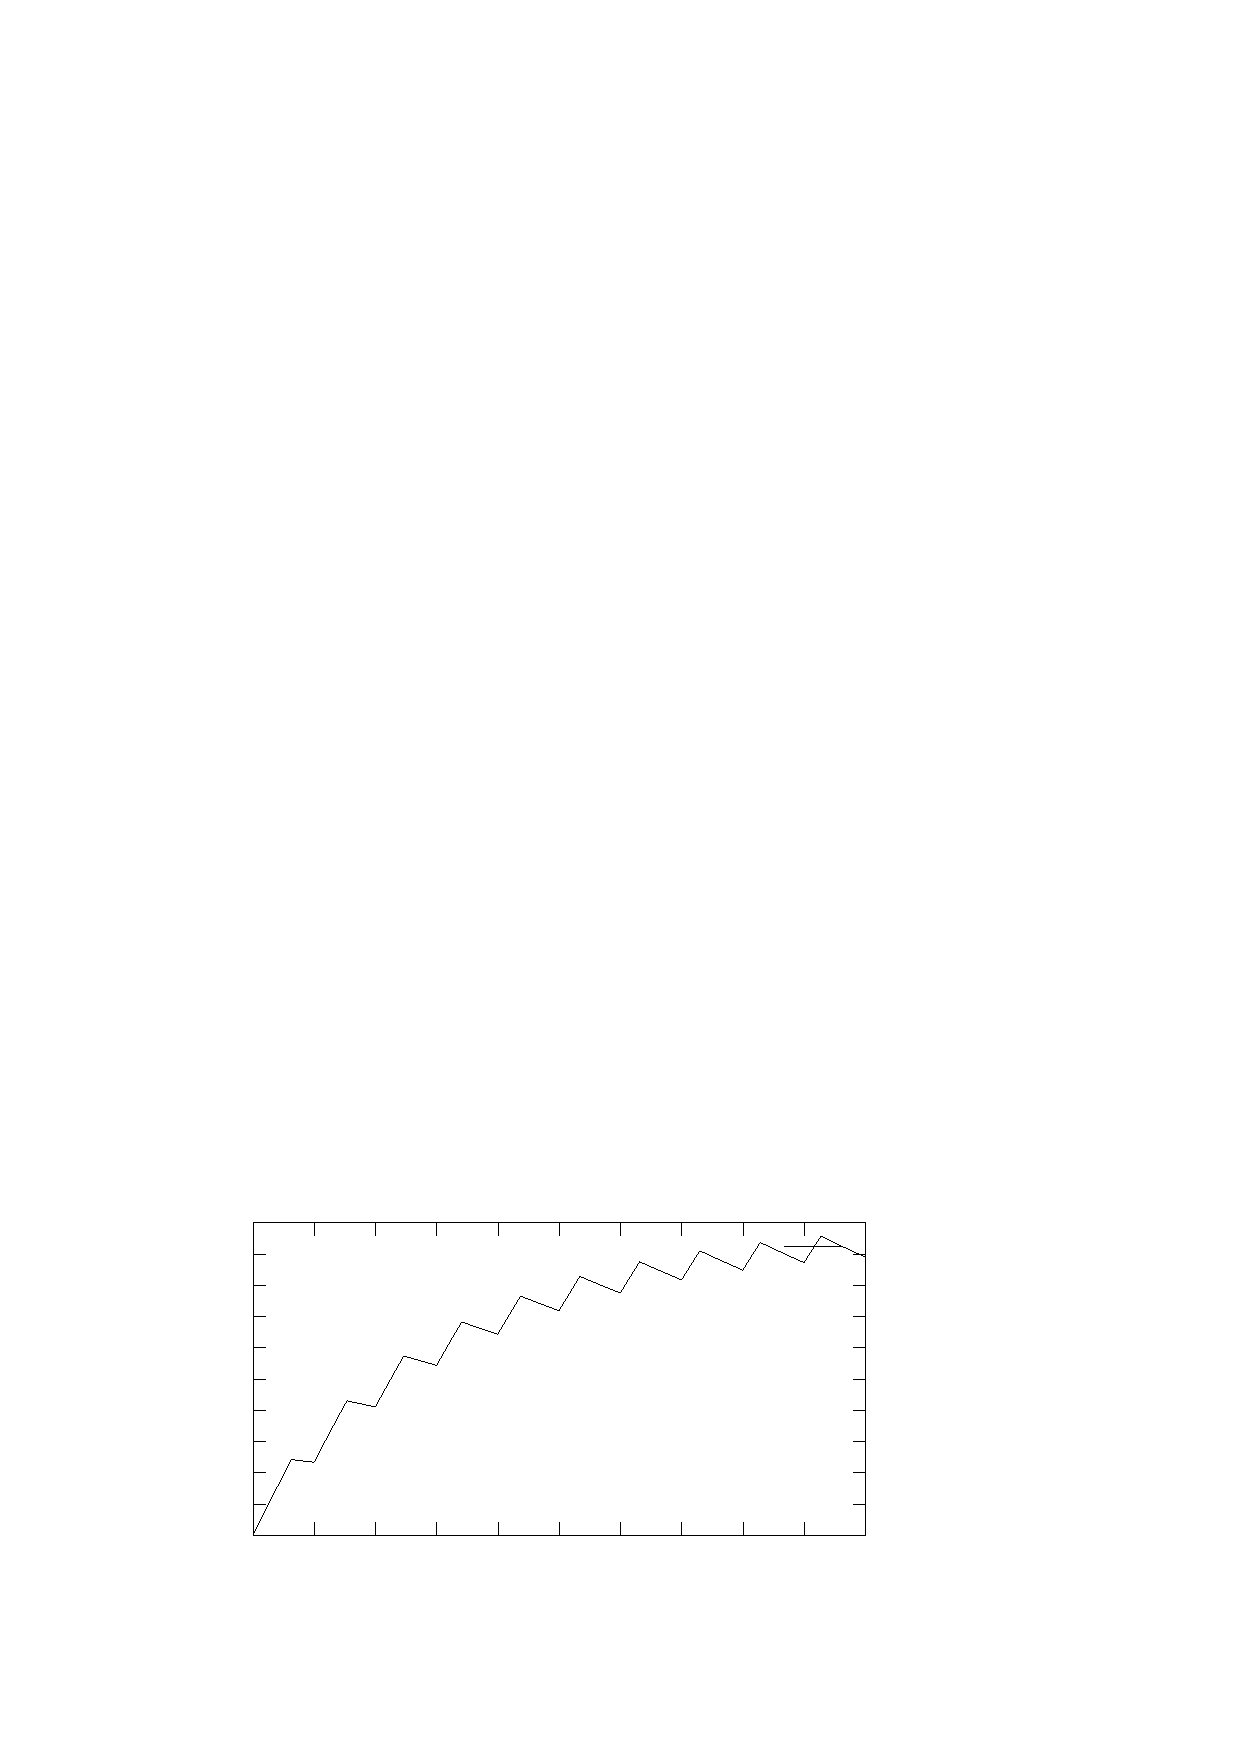
\includegraphics{CS}%
\end{picture}%
\begingroup
\setlength{\unitlength}{0.0200bp}%
\begin{picture}(18000,10800)(0,0)%
\put(2200,1650){\makebox(0,0)[r]{\strut{} 0}}%
\put(2200,2400){\makebox(0,0)[r]{\strut{} 0.5}}%
\put(2200,3150){\makebox(0,0)[r]{\strut{} 1}}%
\put(2200,3900){\makebox(0,0)[r]{\strut{} 1.5}}%
\put(2200,4650){\makebox(0,0)[r]{\strut{} 2}}%
\put(2200,5400){\makebox(0,0)[r]{\strut{} 2.5}}%
\put(2200,6150){\makebox(0,0)[r]{\strut{} 3}}%
\put(2200,6900){\makebox(0,0)[r]{\strut{} 3.5}}%
\put(2200,7650){\makebox(0,0)[r]{\strut{} 4}}%
\put(2200,8400){\makebox(0,0)[r]{\strut{} 4.5}}%
\put(2200,9150){\makebox(0,0)[r]{\strut{} 5}}%
\put(2475,1100){\makebox(0,0){\strut{} 0}}%
\put(3945,1100){\makebox(0,0){\strut{} 200}}%
\put(5415,1100){\makebox(0,0){\strut{} 400}}%
\put(6885,1100){\makebox(0,0){\strut{} 600}}%
\put(8355,1100){\makebox(0,0){\strut{} 800}}%
\put(9825,1100){\makebox(0,0){\strut{} 1000}}%
\put(11295,1100){\makebox(0,0){\strut{} 1200}}%
\put(12765,1100){\makebox(0,0){\strut{} 1400}}%
\put(14235,1100){\makebox(0,0){\strut{} 1600}}%
\put(15705,1100){\makebox(0,0){\strut{} 1800}}%
\put(17175,1100){\makebox(0,0){\strut{} 2000}}%
\put(550,5400){\rotatebox{0}{\makebox(0,0){\strut{}$I_L$}}}%
\put(9825,275){\makebox(0,0){\strut{}time ($10^{-7}s$)}}%
\put(9825,9975){\makebox(0,0){\strut{}switch circuit}}%
\end{picture}%
\endgroup
\endinput

  }
  \caption{A simple switched circuit.}
  \label{fig:figcircuit1}
\end{figure}

\subsection{The dynamical system}
\label{section31}

The dynamics of the circuit in figure \ref{fig:figcircuit1} is obtained using the algorithm of automatic circuit equation formulation.
In a first step, the vector of unknowns is built, in a second step, the dynamical system is
written, and, in a last step, the non-smooth law is added. Applying the automatic equations generation algorithm leads to the following 9-dimensional state vector: $X=(V_1\;V_2\;V_3\;V_4\;I_L\;I_{03}\;I_{04}\;I_s\;I_d)^{T}$, where $V_{1}$ is the voltage across ???, $V_{2}$ is the voltage across ???, $V_{3}$ is the voltage across ???, $V_{4}$ is the voltage across ???, $I_{L}$ is the current through ???, $I_{03}$ is the current through ???, $I_{04}$ is the current through ???, $I_{S}$ is the current through ???, $I_{d}$ is the current through ???.  Building the dynamical equations consists in writing the KCL at each node, the constitutive equation of the smooth branch, and the
non-smooth law of the other branch. The two non-smooth devices are the diode and the switch. It yields the following system, that fits within teh general framework in (\ref{eq:71}): 

\begin{equation}
  \label{eq:72}
 \left\{ \begin{array}{l l l}
    \begin{array}{l}
      L  \frac{dI_L}{dt}(t) = V_1(t)-V_2(t) \\
      I_d(t)+I_s(t)-I_L(t)=0 \\
      I_L(t)-\frac{V_2(t)}{R}=0\\
      I_{03}(t)=0\\
      I_{04}(t)-I_{s}(t)=0\\
      V_4(t)=20\\
      V_3=e(t)\\
\end{array}
& \left.\begin{array}{l}
      \\
      \\ \\ \\ \\
\end{array}\right\}& \text{ Differential-Algebraic Equations}\\ \\[2mm]
  \begin{array}{l}
V_{1}(t)=\frac{1}{2}(\tau_{1}(t)-1)R_\off I_{d}(t)-\frac{1}{2}(\tau_{1}(t)+1) R_\on I_{d}(t) \\ 
V_{1}(t)-V_{4}(t)=\frac{1}{2}(1+\tau_{2}(t)) R_\off I_{s}(t)+\frac{1}{2}(1-\tau_{2}(t)) R_\on I_{s}(t)
  %  0 = V_1(t)-V_4(t)+I_s(t) (\lambda_2+R_\on) \\
  %  0 = V_1(t)+I_d(t)(\lambda_4(t)+R_\on) \\
   % y_1(t) = R_\off-\lambda_2(t)-R_\on\\
   % y_2(t) = V_3(t)-V_2(t)+\lambda_1(t)\\
  %  y_3(t) = R_\off-\lambda_4(t)-R_\on\\
  %  y_4(t) = -V_1(t)+\lambda_3(t) \\
  \end{array} & \left.\begin{array}{c}
     \\ \\
  \end{array}\right\} & \begin{array}{l}
   \text{Input/output relations }\\
   \text{on non-smooth components}
  \end{array}  \\  [5mm]
  \begin{array}{l}
  V_{1}(t) \in - N_{[-1,1]}(\tau_{1}(t)) \\   V_{3}(t)-V_{2}(t) \in -N_{[-1,1]}(\tau_{2}(t))
\end{array} 
& \left.\begin{array}{c} \\ \\ \end{array}\right\}  &  \text{ "Inclusion rule"}\\ 
\end{array}\right.
\end{equation}

\subsection{Numerical results with {\sc siconos}}
\label{section32}

The figure \ref{fig:SIMU_CS} depicts the current evolution through the inductor $L$. In \cite{maffezzoni2006}, it has been shown that the Newton-Raphson algorithm fails when the state of the diode and of the switch changes at $t=t_s$ in figure \ref{fig:SIMU_CS}. Indeed, the linearization performed at each Newton-Raphson iteration leads to an oscillation between two incorrect states and never convergse to the correct one. The Newton-Raphson iterations enter into a infinite loop without converging.  Using the NSDS approach the OSNSP solver converges and computes the correct state. 


 \begin{figure}[h]
 \resizebox{\linewidth}{!}{%GNUPLOT: LaTeX picture with Postscript
\begin{picture}(0,0)%
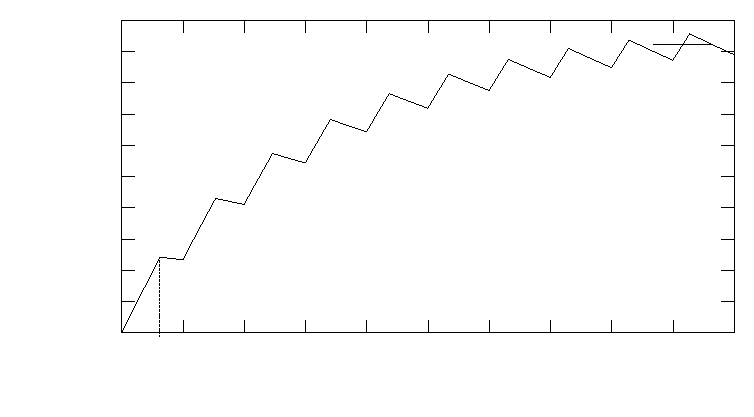
\includegraphics{./figure/simuCS}%
\end{picture}%
\begingroup
\setlength{\unitlength}{0.0200bp}%
\begin{picture}(18000,10800)(0,0)%
\put(2200,1650){\makebox(0,0)[r]{\strut{} 0}}%
\put(2200,2400){\makebox(0,0)[r]{\strut{} 0.5}}%
\put(2200,3150){\makebox(0,0)[r]{\strut{} 1}}%
\put(2200,3900){\makebox(0,0)[r]{\strut{} 1.5}}%
\put(2200,4650){\makebox(0,0)[r]{\strut{} 2}}%
\put(2200,5400){\makebox(0,0)[r]{\strut{} 2.5}}%
\put(2200,6150){\makebox(0,0)[r]{\strut{} 3}}%
\put(2200,6900){\makebox(0,0)[r]{\strut{} 3.5}}%
\put(2200,7650){\makebox(0,0)[r]{\strut{} 4}}%
\put(2200,8400){\makebox(0,0)[r]{\strut{} 4.5}}%
\put(2200,9150){\makebox(0,0)[r]{\strut{} 5}}%
\put(2475,1100){\makebox(0,0){\strut{} 0}}%
\put(3345,1200){\makebox(0,0){\strut{} $t_s$}}%
\put(3945,1100){\makebox(0,0){\strut{} 200}}%
\put(5415,1100){\makebox(0,0){\strut{} 400}}%
\put(6885,1100){\makebox(0,0){\strut{} 600}}%
\put(8355,1100){\makebox(0,0){\strut{} 800}}%
\put(9825,1100){\makebox(0,0){\strut{} 1000}}%
\put(11295,1100){\makebox(0,0){\strut{} 1200}}%
\put(12765,1100){\makebox(0,0){\strut{} 1400}}%
\put(14235,1100){\makebox(0,0){\strut{} 1600}}%
\put(15705,1100){\makebox(0,0){\strut{} 1800}}%
\put(17175,1100){\makebox(0,0){\strut{} 2000}}%
\put(550,5400){\rotatebox{0}{\makebox(0,0){\strut{}$I_L$}}}%
\put(9825,275){\makebox(0,0){\strut{}time ($10^{-7}s$)}}%
\put(9825,9975){\makebox(0,0){\strut{}switched circuit}}%
\end{picture}%
\endgroup
\endinput
 }
  \label{fig:SIMU_CS}
\caption{Current through the inductor.}
 \end{figure}


\begin{remark}
In \cite{maffezzoni2006} an event-driven numerical method is proposed to solve the non convergence issue. However it is reliable only if the switching times can be precisely estimated, a shortcoming not encountered  with the NSDS and the  Moreau's time-stepping method. 
\end{remark}

\section{Results on the buck converter}
\label{section4}


\begin{figure*}[!ht]
\centerline{
 \scalebox{1.0}{
    \input{./figure/buck.pstex_t}
 }
}
\caption{Buck converter}
\label{fig-Buck-converter}
\end{figure*}
The components are modelled with either linear or piecewise linear or set-valued relations yielding a non-smooth dynamical system of the linear time invariant complementarity systems class. The features of these models are given thereafter:

\paragraph{Power MOSFETS pMOS/nMOS:} 





they are described as an assembly of a
piecewise-linear current source $I_{DS} = f(V_{GS}, V_{DS})$ and the intrinsic diode
(DPMOS and DNMOS) with an ideal characteristic.
The capacitances were not taken into account. The diodes threshold is
1 V. The MOSFETs transconductance KP was set to $10 AV^{-2}$ and
their threshold voltage to respectively -2 V for the PMOS and 2 V for
the NMOS. One can notice that the sum of their absolute values largely
exceeds the supply voltage $V_{I} = 3 V$ , thus providing non-overlapping
conduction times.

The relative error between $f(\cdot)$ and $f_\pwl(\cdot)$ is kept below $0.1$ for $0.1 \leq x < 3.82$. The absolute error is less than $2 \cdot 10^{-3}$ for $0 \leq x < 0.1$ and $0$ for negative $x$. In practice, the values of $V_G,V_S,V_D,V_T$ in logic integrated circuits allow  a good approximation of $f(\cdot)$ by $f_\pwl(\cdot)$. Obviously it is possible to describe the function $f(\cdot)$ with less segments, however a study of the results accuracy and computation time as a function of the number of segments is outside the scope of this paper. 
(sample values of $750~cm^2.V^{-1}.s^{-1}$ for a NMOS, $250~cm^2.V^{-1}.s^{-1}$ for a pMOS), $C_{OX} = \frac{\epsilon_{SiO_2}}{t_{OX}}$, $\epsilon_{SiO_2} = \epsilon_{r~SiO_2} \cdot \epsilon_0 \ (\epsilon_{r~SiO_2} \approx 3.9)$, $t_{OX}$ oxide thickness $\approx 4 nm$ in a recent $180 nm$ technology, $W$ channel width, $L$ channel length $\approx 130 nm$ in a recent $180 nm$ technology, $V_T$ threshold voltage depending on technology, $V_{BS}$ , temperature $\approx 0.25$ to $1$ V

\begin{equation}
  \label{eq:70}
 \left\{ \begin{array}{l}
  b = \frac{K}{2} \\
  c_1 = 0.09 , c_2=0.2238 , c_3=0.4666 , c_4=1.1605 , c_5=2.8863 \\
  h_i = b(V_T+a_i), i =1\ldots 5 \\
  a_1 = 0 , a_2=0.1, a_3=0.2487 , a_4=0.6182 , a_5=1.5383 \\
\end{array}\right.
\end{equation}

\paragraph{Compensator amplifier:} is modelled as a 10000 gain and an output low-pass
filter with a cutoff frequency of 30 MHz.
\paragraph{Comparator:} is modelled as a piecewise-linear function whose value is 0 if
$x < -0.15V$ and 3 if $x > 0.15V$ .
\paragraph{Ramp voltage:} the frequency is 600 kHz and the bounds are 0 and 0.75 VI = 2.25 V .
The rise time is 1.655 ns and the fall time is 10 ns.
\paragraph{Other components:} $V_I = 3 V , L = 10 \micro H, C = 22 \micro F,R_{load} = 10,$ compensator
: $R_{11} = 15.58 \kilo \ohm , R_{12} = 227.8 \kilo \ohm ,R_{21} = 5.613 \mega \ohm, C_{11} = 20 \pico F, C_{21} =
1.9 \pico F$
The reference voltage Vref rises from 0 to 1.8 V in 0.1 ms at the beginning
of the simulation.
The output voltage Voutput is regulated to track the reference voltage Vref when
VI or Vref or the load current vary. The error voltage Verror is a filtered value
of the difference between Voutput and Vref . This voltage signal is converted
into a time length thanks to a comparison with the periodic ramp signal. The
comparator drives the PMOS transistor which in turn provides more or less
charge to the output depending on the error level. The operation of a buck
converter involves both a relatively slow dynamics when the switching elements
(MOS and diodes) are keeping their conducting state, and a fast dynamics when
the states change. The order of magnitude are $ 50 \pico s$ for some switching details,
1 us for a slow variation period and $100 \micro s$ at least for a settling period of the
whole circuit requiring a simulation.

\subsection{The dynamical equations}
\label{section41}
The non-smooth DAE has been generated using the automatic circuit equation formulation describde in figure
\ref{fig:acef_algo}. It leads to a dynamical system with 25 states coupled to an inclusion rule. The dimension of the inclusion
rule depends on the MOS model. It is 12 with a approximation of 2 segments, or 24 using the
model in \ref{eq:68}.  

\subsection{Numerical results with {\sc siconos},  and comparisons}
\label{section42}
\subsubsection{Simulation with SICONOS}
 The start-up of the converter was simulated thanks to the {\sc siconos} platform
developed at INRIA. As initial conditions, all state variables are zeroed.
The detailed analysis of the switching events requires to use a time step as
small as $50 \pico s$. The simulations are carried with a fixed time step, 4000000 steps
are then computed for the $200 \micro s$ long settling of the output voltage.
The overall result is shown on the figure \ref{fig:figSimuBuck}.  
\vskip 0.2cm
{\bf Simulation time:} The CPU time required to achieve the simulation is 60 seconds on a
Pentium 4 processor clocked at 3 GHz. It includes 19 seconds in the MLCP solvers, 40 seconds in
matrix products. The time to export the resulting data is not included.
\begin{figure}[h]
  \centering
   \scalebox{0.6}{
  \input{./figure/BuckSimu.pstex_t}
  }
  \caption{Buck converter simulation.}
  \label{fig:figSimuBuck}
\end{figure}

\begin{enumerate}
  \item[--] The figure \ref{fig:figSimuBuck} (a) is the output potential, following the ramp $V_{ref}$.
    \item[--] The figure \ref{fig:figSimuBuck} (b) is the current through the inductor. Until $0.0001s$, $I_L$
    is loading the capacitor C. After $0.0001s$, $I_L$ has to keep constant the capacitor charge.
    \item[--] The figure \ref{fig:figSimuBuck} (c) zooms on the pMOS drain potential with standard
    parameters.
    \item[--] The figure  \ref{fig:figSimuBuck} (d) zooms on the pMOS drain potential with, $L=4\micro H,
    C=10\micro F,
    R_{11}=10\kilo \ohm, R_{21}=8\kilo \ohm ,C_{11}=10\pico F$, exhibiting a
    sliding mode that is smoothly simulated. 
  \end{enumerate}

The simulation has been tested with many parameters values. The robustness of the non-smooth modelling and solving algorithms enables to perform with the same CPU time the simulation of such cases. The method has been tested with variations in the MOSFET transistors piecewise-linear approximations (6 or 2 segments), and with the multivalued and the regularized comparator models. No significant changes on the numerical results were noticed, indicating that the main objective is the reduction of the variables number (the MLCP size).  



\subsubsection{Simulation with SPICE }

\paragraph{Simulation conditions: convergence issues related to the MOS model}
The simulation of this circuit was done with several versions of SPICE (the open source NGSPICE from Berkeley, SMASH from Dolphin \footnote{http://www.dolphin.fr/medal/smash/smash$\_$overview.php} and ELDO from Mentor Graphics) and two kinds of MOS models :
\begin{description}
\item[the MOS level 3 model :] this model was preferred to the MOS level 1 since it allowed the convergence
of the SMASH simulator with the requirement to add a small capacitor between ground and node 2 (connection between
the MOS transistors). This model takes more physical effects into account than the piecewise linear model used in SICONOS simulations,
in particular the voltage-dependent capacitances. It is an important issue since these varying capacitances
cause some convergence problems when node 2 switches between $V_I$ and ground.
Adding a small capacitor of a few picoFarad between this node and ground helps to solve the problem
but may yield artifacts (spikes) on the current of the~$V_I$~alim and the MOS transistors.
\item[a simplified model (Sah model)] with fixed capacitances and a quadratic static characteristic :
\[
I_{DS} = \textrm{max}(0,V_{GS}-Vt_N)^2 - \textrm{max}(0,V_{GD}-Vt_N)^2 \qquad \textrm{for an nMOS}
\]
This model is very close to the piecewise linear model used in {\sc siconos} simulations. The implementation in netlists was done thanks to 
voltage-dependent current sources that are very likely not compiled by the various SPICE simulators tested.
Thus the CPU time measured is increased with respect to a compiled version of the same model.
An estimation of the CPU time with a compiled simplified model is given by multiplying the MOS level 3 CPU time
by the ratio of the Newton-Raphson iterations required respectively during the simulations with each model.
An additional correction should be done to reflect that the computation of the jacobian matrix entries
linked to a compiled simplified model would require less time than with a MOS level 3 model. Even if the SPICE simulation
includes other operations, jacobian matrix loading time is indeed known to be generally predominant.
\end{description}


\begin{itemize}
\item Power MOSFETS intrinsic diodes are modelled by the classical Shockley equation with an emission
coefficient $N~=~1$ :
\[ I = I_S.({e^{\frac{q.V}{N.k.T}} - 1}) \qquad \textrm{when} \quad V > -5.N.\frac{k.T}{q} \]
\[ I = -I_S \qquad  \textrm{when} \quad V < -5.N.\frac{k.T}{q} \]
with
\[
\begin{array}{ll}
V\,,\,I & \textrm{voltage across the diode and current through the diode}\\
I_S & \textrm{saturation current, default value $10^{-14}$~A}\\
q & \textrm{electron charge $1.6\,10^{-19}$~C}\\
k & \textrm{Boltzmann constant $1.38\,10^{-23}\,J.K^{-1}$}\\
T & \textrm{temperature in K}\\
N & \textrm{emission coefficient}
\end{array}
\]
\item The comparator is modelled as a non linear voltage controlled voltage source defined as $V_{out}~=~1.5~\cdot~(tanh(10~\cdot~V_{in}) + 1)$. Thus the 3~segment characteristic used as the non-smooth model is regularized to help convergence of SPICE
(see a comparison of the piecewise-linear comparator as used in {\sc siconos} simulations with the SPICE one in figure \ref{fig-comparator-models}).
\end{itemize}

\begin{figure}[hbtp]
\begin{center}
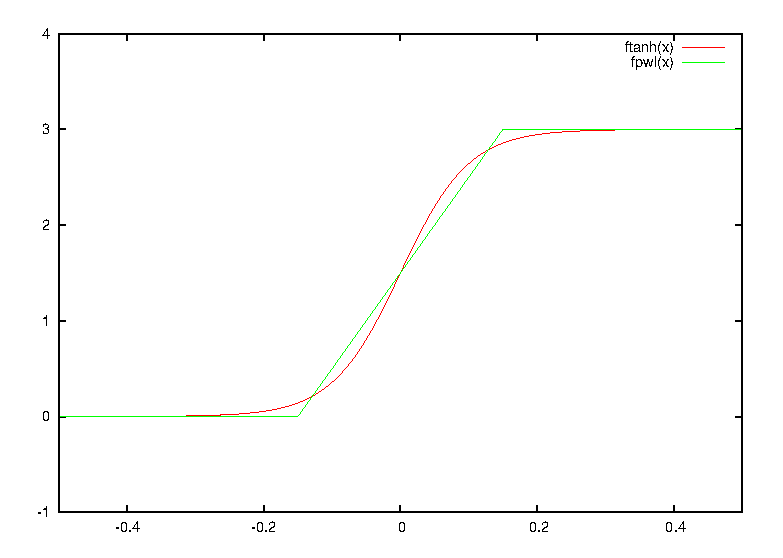
\includegraphics[scale=0.6,angle=0]{./figure/comparators.eps}
\end{center}
\caption{Comparison of piecewise-linear and SPICE (tanh based) comparator models.}
\label{fig-comparator-models}
\end{figure}



The power supply $V_I$ is raised from 0 in $50~ns$ at the beginning to help the convergence.\footnote{This is
not required with the {\sc siconos} algorithms that find a consistent initial solution from scratch.}
The SPICE tolerance values used are $1~nA$ for currents, $1~\mu V$ for voltages and $0.00075$ for relative differences.
The maximum number of Newton-Raphson iterations is set to 100 (the default values are 10 for NGSPICE, 20 for SMASH and
13 for ELDO).

Usually, SPICE simulators integrate time with a time step adjusted according to different strategies based on an estimation
of the local truncation error (LTE) or the number of Newton-Raphson iterations required by previous steps.
Since {\sc siconos} simulations were carried with a fixed time step of~50~ps, simulators were forced to use this value as a maximum.
Even when SPICE simulators use fixed time step, they may compute LTE to assess a solution found by the Newton-Raphson
algorithm. This computation of LTE was disabled because it could impair the performance of SPICE with respect to {\sc siconos}.
\footnote{For NGSPICE, it implied a slight modification of the source code since no standard option is provided to do it.}

\subsubsection{Simulation comparisons}
The following tables displays the results with the standard and the sliding mode values of compensator components. An estimation of the CPU time with a compiled simplified model is added.
\\
\\
\begin{tabular}{|l|c|r|r|r|r|}
\hline
\multicolumn{6}{|c|}{\textbf{standard compensator values}}\\
\hline
simulator & model & time steps & NR iterations & CPU time (s) & CPU time estimation (s)\\
\hline
NGSPICE & simple  & 4000000 & 8024814 & 632 & 357\\
NGSPICE & level 3 & 4000000 & 8304237 & 370 & \\
\hline
SMASH   & simple  & 4000404 & 8073070 & 230 & 172\\
SMASH   & level 3 & 4000323 & 8059868 & 172 & \\
\hline
ELDO    & simple  & 4000000 & 4547579 & 388 & 355\\
ELDO    & level 3 & 4000000 & 4554452 & 356 & \\
\hline
\end{tabular}\\
\begin{tabular}{|l|c|r|r|r|r|}
\hline
\multicolumn{6}{|c|}{\textbf{sliding mode compensator values}}\\
\hline
simulator & model & time steps & NR iterations & CPU time (s) & CPU time estimation (s)\\
\hline
NGSPICE & simple  & 4000000 & 8070324 & 638 & 358\\
NGSPICE & level 3 & 4000000 & 8669053 & 385 & \\
\hline
SMASH   & simple  & 4000252 & 8239697 & 234 & 176\\
SMASH   & level 3 & 4000131 & 8220181 & 176 & \\
\hline
ELDO    & simple  & 4000000 & 5861226 & 438 & 365\\
ELDO    & level 3 & 4000000 & 5888994 & 367 & \\
\hline
\end{tabular}
\\
\\
These results shall be compared to the 60~s~CPU time achieved with the non-smooth dynamics.
Depending on the model and the SPICE simulator, the (estimated) CPU time is from~2.8~to~6.1
larger than with SICONOS.\\

Moreover, it was necessary to add a parasitic capacitor on the connection between the PMOS and NMOS
transistors to allow the convergence of the SMASH simulator with both models of MOS
and of the NGSPICE simulator with the MOS level 3 model.


\subsubsection{Simulation with PLECS}

As we pointed out above, the hybrid approach that consists of an exhaustive enumeration of all the system's modes, soon become inefficient and unusable mainly because the simulation duration grows exponentially fast. Let us illustrate this fact with the buck converter, loaded with several devices: a resistance, and a chain of transistors. The simulator is PLECS, a hybrid simulator developed by Plexim \footnote{http://www.plexim.com/}. 




\section{Conclusions}
\label{section5}


In this paper we have presented numerical simulations of switched circuits obtained with a suitable time-stepping implicit method, named Moreau's time-stepping algorithm. This method is based on the non-smooth dynamical systems modelling approach, and relies heavily on complementarity problems (equivalently, inclusions into normal cones) solvers. The advantages of such a method are that it allows one to:

\begin{itemize}

\item avoid computing the dynamics changes due to topology variations, since the circuits are treated as a global system with a fixed state dimension; modes transitions are taken care of by the complementarity problem solvers, which usually are polynomial in time;

\item simulate circuits with very large number of events without slowing down too much the simulation;

\item avoid regularization and consequently stiff systems of ODEs;

\item accurately calculate the initial steady-state of the system;

\item accurately simulate sliding mode trajectories without spurious oscillations around the switching surface;

\item compute state jumps (initial jumps due to inconsistent states, or in the course of the integration). 

\end{itemize}


The major drawback of the used method is its low order, so that its accuracy may be less good on smooth portions of the trajectoires. In this paper it is first shown that Moreau's time stepping scheme allows one to integrate an academic example on which Newton-Raphson based methods fail. Then the buck converter system is simulated. Comparisons with other analog simulators are presented. The simulations have been led with the {\sc siconos} software package of the INRIA, an open source platform dedicated to non-smooth multivalued dynamical systems. 




%%% Local Variables: 
%%% mode: latex
%%% TeX-master: "IEEEpaper"
%%% End: 
